\documentclass[aspectratio=169]{beamer}

% Theme and color scheme
\usetheme{Madrid}
\usecolortheme{default}

% Custom colors
\definecolor{rocketblue}{RGB}{0, 51, 102}
\definecolor{rocketorange}{RGB}{255, 140, 0}
\definecolor{rocketgray}{RGB}{64, 64, 64}

\setbeamercolor{structure}{fg=rocketblue}
\setbeamercolor{title}{fg=rocketblue}
\setbeamercolor{frametitle}{fg=rocketblue}

% Remove navigation symbols
\setbeamertemplate{navigation symbols}{}

% Custom footer
\setbeamertemplate{footline}{
  \hfill
  \insertframenumber/\inserttotalframenumber
  \hspace{1em}\vspace{1em}
}

% Packages
\usepackage{graphicx}
\usepackage{tikz}
\usepackage{fontawesome5}
\usepackage{multicol}

% Title information
\title[Autonomous Rocket Landing]{Autonomous Rocket Landing\\with Reinforcement Learning}
\author{Ryan Christ \& Jay Parmar}
\institute{Duke University}
\date{CS 372 Final Project}

\begin{document}

% Title slide
\begin{frame}
\begin{center}
\vspace{1.5em}

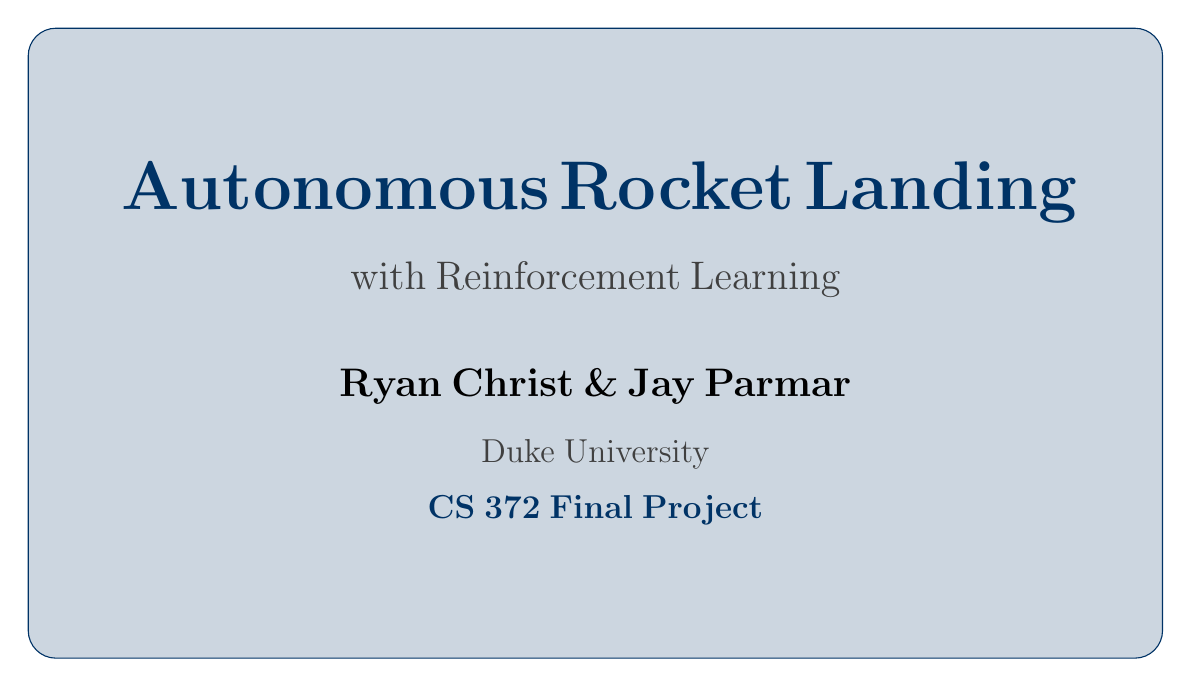
\begin{tikzpicture}
% Blue box background
\node[draw=rocketblue, fill=rocketblue!20, rounded corners=10pt, text width=13cm, align=center, inner sep=2em, minimum height=8cm] (box) {
    \vspace{0.5em}
    {\Huge\textcolor{rocketblue}{\textbf{Autonomous Rocket Landing}}}
    
    \vspace{0.8em}
    {\Large\textcolor{rocketgray}{with Reinforcement Learning}}
    
    \vspace{2.5em}
    
    {\Large\textbf{Ryan Christ \& Jay Parmar}}
    
    \vspace{1.2em}
    
    {\large\textcolor{rocketgray}{Duke University}}
    
    \vspace{0.8em}
    
    {\large\textcolor{rocketblue}{\textbf{CS 372 Final Project}}}
    
    \vspace{0.5em}
};
\end{tikzpicture}

\vspace{1em}

{\Large\faRocket}

\end{center}
\end{frame}

% ============================================
% SECTION 1: Problem Motivation
% ============================================
\section{The Challenge}

\begin{frame}{The Real-World Problem}
\begin{center}
\Large
\textbf{Rocket Landing: One of the Most Challenging Problems\\in Aerospace Engineering}
\vspace{1em}

\begin{tikzpicture}
% Landing pad
\draw[fill=yellow!30, draw=black, thick] (-2, -1) rectangle (2, -0.5);
\node at (0, -0.75) {\textbf{Landing Pad}};

% Rocket trajectory
\draw[->, thick, rocketblue] (3, 3) .. controls (1, 1.5) .. (0, -0.3);
\node at (3.5, 3.2) {\faRocket};

% Objectives
\node[align=left] at (-4, 1.5) {
    \textbf{Key Objectives:}\\
    \faCheckCircle\ Safety\\
    \faCheckCircle\ Fuel Efficiency\\
    \faCheckCircle\ Precision
};
\end{tikzpicture}

\small
\textit{Critical for reusable rocket technology\\where autonomous landing systems are essential}
\end{center}
\end{frame}

\begin{frame}{Our Unified Goal}
\begin{center}
\Huge
\textcolor{rocketblue}{\textbf{Our Project Goal}}
\vspace{1em}

\Large
To develop and compare reinforcement learning algorithms\\
that can autonomously land a rocket\\
safely and efficiently

\vspace{1em}

\begin{tikzpicture}
\node[draw, rounded corners, fill=rocketblue!20, text width=8cm, align=center, padding=1em] {
    \large\textbf{Real-World Application}\\
    \normalsize
    Addresses a critical challenge in aerospace engineering\\
    Relevant to SpaceX, Blue Origin, and future space missions
};
\end{tikzpicture}
\end{center}
\end{frame}

% ============================================
% SECTION 2: What We Built
% ============================================
\section{Our Solution}

\begin{frame}{What We Built}
\begin{center}
\Huge
\textcolor{rocketblue}{\textbf{AI-Powered Rocket Landing System}}
\vspace{1em}

\Large
An intelligent agent that learns to land rockets autonomously

\vspace{1.5em}

\begin{columns}
\begin{column}{0.5\textwidth}
\begin{center}
\textbf{Live Demonstration}
\vspace{0.5em}

\small
\texttt{python src/scripts/test\_visual.py}\\
\texttt{--algorithm dqn}\\
\texttt{--checkpoint models/dqn/}\\
\texttt{dqn\_adam\_best.pt}
\end{center}
\end{column}

\begin{column}{0.5\textwidth}
\begin{center}
\textbf{Key Capabilities}
\vspace{0.5em}

\begin{itemize}
\item Starts from random positions
\item Navigates to landing pad
\item Controls rocket engines
\item Learns fuel-efficient strategies
\end{itemize}
\end{center}
\end{column}
\end{columns}
\end{center}
\end{frame}

\begin{frame}{Two AI Approaches}
\begin{center}
\Large
\textbf{We Compared Two Different AI Methods}
\vspace{1.5em}

\begin{columns}
\begin{column}{0.5\textwidth}
\begin{center}
\textbf{DQN}\\
\textit{Deep Q-Network}
\vspace{0.5em}

\begin{tikzpicture}
\node[draw, rounded corners, fill=rocketblue!20, text width=5cm, align=center, padding=0.5em] {
    \small
    Learns by estimating\\
    the value of actions\\
    \vspace{0.3em}
    \faLightbulb\ Value-based approach
};
\end{tikzpicture}
\end{center}
\end{column}

\begin{column}{0.5\textwidth}
\begin{center}
\textbf{A2C}\\
\textit{Actor-Critic}
\vspace{0.5em}

\begin{tikzpicture}
\node[draw, rounded corners, fill=rocketorange!20, text width=5cm, align=center, padding=0.5em] {
    \small
    Learns a policy directly\\
    through experience\\
    \vspace{0.3em}
    \faLightbulb\ Policy-based approach
};
\end{tikzpicture}
\end{center}
\end{column}
\end{columns}

\vspace{1.5em}
\large
\textbf{Both Successfully Learn to Land Rockets}
\end{center}
\end{frame}

\begin{frame}{Performance Results (Test Set, 50 eps, with reward wrapper)}
\Large
\textbf{Quantitative outcomes from \texttt{results/test\_results.csv}}
\vspace{0.8em}

\begin{center}
\small
\begin{tabular}{lccc}
\textbf{Agent} & \textbf{Mean Return} & \textbf{Success} & \textbf{Fuel} \\
\hline
DQN (Adam) & 373.6 $\pm$ 21.6 & 100\% & 75.9 \\
DQN (RMSprop) & 366.2 $\pm$ 19.6 & 100\% & 92.3 \\
A2C (Adam) & 225.9 $\pm$ 202.2 & 64\% & 58.1 \\
A2C (SGD) & -85.0 $\pm$ 191.8 & 28\% & 232.4 \\
\end{tabular}
\end{center}

\vspace{0.6em}
\normalsize
\begin{itemize}
    \item[\faCheckCircle] DQN achieves perfect success; Adam slightly more efficient than RMSprop.
    \item[\faCheckCircle] A2C works with Adam but underperforms DQN; SGD fails to converge.
    \item[\faCheckCircle] Fuel efficiency trade-off: A2C (Adam) uses least fuel but has lower success.
\end{itemize}
\end{frame}

% ============================================
% SECTION 3: Key Features
% ============================================
\section{Key Features}

\begin{frame}{Optimizer Comparison (DQN \& A2C)}
\begin{columns}
\begin{column}{0.5\textwidth}
\textbf{DQN (Adam vs RMSprop)}
\begin{itemize}
    \item Mean return: 373.6 vs 366.2
    \item Success: both 100\%
    \item Fuel: 75.9 vs 92.3 (Adam more efficient)
    \item Episode length: 198 vs 220 (Adam shorter)
\end{itemize}
\textit{[Placeholder: insert small bar chart]}\\
\scriptsize \texttt{data/plots/dqn\_adam\_learning\_curve.png}, \texttt{dqn\_rmsprop\_learning\_curve.png}
\end{column}
\begin{column}{0.5\textwidth}
\textbf{A2C (Adam vs SGD)}
\begin{itemize}
    \item Mean return: 225.9 vs -85.0
    \item Success: 64\% vs 28\%
    \item Fuel: 58.1 vs 232.4 (Adam 4x better)
    \item Crash rate: 36\% vs 70\%
\end{itemize}
\textit{[Placeholder: insert small bar chart]}\\
\scriptsize \texttt{data/plots/a2c\_adam\_learning\_curve.png}, \texttt{a2c\_sgd\_learning\_curve.png}
\end{column}
\end{columns}
\end{frame}

% ============================================
% SECTION 4: Why It Matters
% ============================================
\section{Impact}

\begin{frame}{Why This Matters}
\begin{center}
\Huge
\textcolor{rocketblue}{\textbf{Real-World Applications}}
\vspace{1.5em}

\begin{columns}
\begin{column}{0.33\textwidth}
\begin{center}
\faSpaceShuttle\\
\vspace{0.5em}
\textbf{Space Exploration}\\
\small
Autonomous spacecraft landing\\
Lunar and Mars missions
\end{center}
\end{column}

\begin{column}{0.33\textwidth}
\begin{center}
\faHelicopter\\
\vspace{0.5em}
\textbf{Autonomous Systems}\\
\small
Drone navigation\\
Precision control systems
\end{center}
\end{column}

\begin{column}{0.33\textwidth}
\begin{center}
\faDollarSign\\
\vspace{0.5em}
\textbf{Cost Reduction}\\
\small
Reusable rocket technology\\
Economic viability
\end{center}
\end{column}
\end{columns}
\end{center}
\end{frame}

\begin{frame}{Broader Impact}
\begin{center}
\Large
\textbf{Modern AI Techniques Solving Complex Problems}
\vspace{1.5em}

\begin{tikzpicture}
\node[draw, rounded corners, fill=rocketblue!20, text width=11cm, align=left, padding=1em] {
    \large\textbf{The Same Techniques Power:}\\
    \vspace{0.5em}
    \begin{itemize}
    \item[\faRobot] Advanced robotics systems
    \item[\faCar] Autonomous vehicles
    \item[\faIndustry] Industrial automation
    \item[\faGamepad] Game AI and strategy
    \end{itemize}
};
\end{tikzpicture}

\vspace{2em}

\large
\textbf{By showing AI can learn to balance safety and efficiency,\\
we're advancing the state of autonomous systems}
\end{center}
\end{frame}

% ============================================
% SECTION 5: Closing
% ============================================
\section{Conclusion}

\begin{frame}{Summary}
\begin{center}
\Huge
\textcolor{rocketblue}{\textbf{Project Summary}}
\vspace{1.5em}

\Large
Reinforcement learning can successfully solve\\
the rocket landing problem

\vspace{1em}

\begin{columns}
\begin{column}{0.5\textwidth}
\begin{center}
\textbf{Achievements}
\vspace{0.5em}

\begin{itemize}
\item[\faCheckCircle] Safe landings
\item[\faCheckCircle] Fuel efficiency
\item[\faCheckCircle] Two AI approaches
\item[\faCheckCircle] Real-world relevance
\end{itemize}
\end{center}
\end{column}

\begin{column}{0.5\textwidth}
\begin{center}
\textbf{Impact}
\vspace{0.5em}

\begin{itemize}
\item[\faRocket] Aerospace applications
\item[\faLightbulb] AI research contribution
\item[\faCode] Open-source codebase
\item[\faGraduationCap] Educational value
\end{itemize}
\end{center}
\end{column}
\end{columns}
\end{center}
\end{frame}

\begin{frame}{Thank You}
\begin{center}
\Huge
\textcolor{rocketblue}{\textbf{Thank You!}}
\vspace{2em}

\Large
\textbf{Ryan Christ \& Jay Parmar}\\
\vspace{0.5em}
\large
Duke University\\
CS 372 Final Project
\vspace{2em}

\large
\textbf{Project Repository}\\
\vspace{0.5em}
\small
\texttt{github.com/[your-repo-url]}

\vspace{2em}
\end{center}
\end{frame}

\end{document}

